% The two k x k matrices of the projected eigenproblem, S and M.
% Time runs vertically as in imgs/echo_strip.tex. The left chain enters as a bra, with no
% complex conjugation.
%
% Standalone: compiles to imgs/projection.pdf.
% Inline:     with \usepackage{standalone}, % The two k x k matrices of the projected eigenproblem, S and M.
% Time runs vertically as in imgs/echo_strip.tex. The left chain enters as a bra, with no
% complex conjugation.
%
% Standalone: compiles to imgs/projection.pdf.
% Inline:     with \usepackage{standalone}, % The two k x k matrices of the projected eigenproblem, S and M.
% Time runs vertically as in imgs/echo_strip.tex. The left chain enters as a bra, with no
% complex conjugation.
%
% Standalone: compiles to imgs/projection.pdf.
% Inline:     with \usepackage{standalone}, % The two k x k matrices of the projected eigenproblem, S and M.
% Time runs vertically as in imgs/echo_strip.tex. The left chain enters as a bra, with no
% complex conjugation.
%
% Standalone: compiles to imgs/projection.pdf.
% Inline:     with \usepackage{standalone}, \input{imgs/projection}.
\documentclass[tikz,border=3pt]{standalone}
\usepackage{amsmath,amssymb,braket,graphicx}
\usetikzlibrary{arrows.meta}

\definecolor{tnL}{RGB}{243,116,63}
\definecolor{tnR}{RGB}{60,110,150}
\definecolor{tnE}{RGB}{250,200,70}

\newcommand{\DY}{0.72}    % time-site spacing
\newcommand{\CS}{0.84}    % column spacing
\newcommand{\LG}{0.42}

\begin{document}
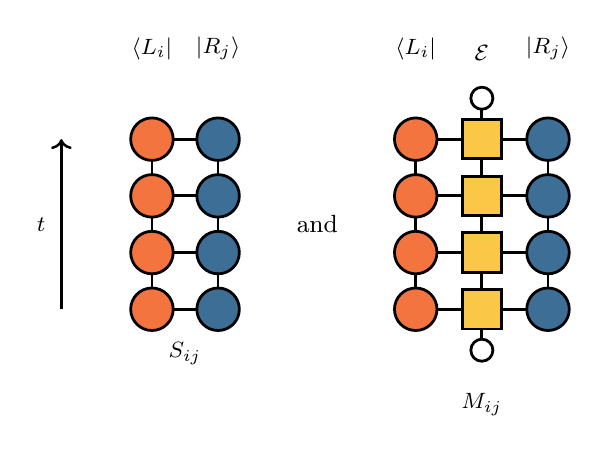
\begin{tikzpicture}[
    bond/.style={draw=black, line width=1.0pt},
    fat/.style={draw=black, line width=2.4pt},
    T/.style={circle, draw=black, line width=1.0pt, minimum size=5.4mm, inner sep=0pt},
    W/.style={rectangle, draw=black, line width=1.0pt, fill=tnE, minimum size=5.0mm, inner sep=0pt},
    P/.style={circle, draw=black, line width=1.0pt, fill=white, minimum size=2.8mm, inner sep=0pt},
    tag/.style={font=\small},
    idx/.style={font=\footnotesize},
  ]

  % product-state caps closing the tMPO column
  \newcommand{\caps}[1]{%
    \draw[bond] (#1,{1.5*\DY}) -- (#1,{1.5*\DY+0.52});
    \draw[bond] (#1,{-1.5*\DY}) -- (#1,{-1.5*\DY-0.52});
    \node[P] at (#1,{1.5*\DY+0.52}) {};
    \node[P] at (#1,{-1.5*\DY-0.52}) {};}

  % temporal MPS: #1 x, #2 fill, #3 leg side
  \newcommand{\tmps}[3]{%
    \draw[bond] (#1,{1.5*\DY}) -- (#1,{-1.5*\DY});
    \foreach \j in {-1.5,-0.5,0.5,1.5} {
      \draw[bond] (#1,{\j*\DY}) -- ({#1+(#3)*\LG},{\j*\DY});
      \node[T, fill=#2] at (#1,{\j*\DY}) {};
    }}

  % transfer-matrix column: legs on both sides, capped
  \newcommand{\tmpo}[1]{%
    \caps{#1}
    \draw[bond] (#1,{1.5*\DY}) -- (#1,{-1.5*\DY});
    \foreach \j in {-1.5,-0.5,0.5,1.5} {
      \draw[bond] ({#1-\LG},{\j*\DY}) -- ({#1+\LG},{\j*\DY});
      \node[W] at (#1,{\j*\DY}) {};
    }}

  % time axis: same direction as imgs/echo_strip.tex
  \draw[->, line width=0.9pt] (-1.15,{-1.5*\DY}) -- (-1.15,{1.5*\DY})
        node[midway, left=2pt, idx] {$t$};

  \tmps{0}{tnL}{1} \tmps{\CS}{tnR}{-1}
  \node[idx, anchor=south] at (0,{1.5*\DY+0.88})   {$\bra{L_i}$};
  \node[idx, anchor=south] at (\CS,{1.5*\DY+0.88}) {$\ket{R_j}$};
  \node[idx, anchor=north] at (0.42,{-1.5*\DY-0.30}) {$S_{ij}$};

  \node[tag] at (2.10,0) {and};

  \tmps{3.35}{tnL}{1} \tmpo{4.19} \tmps{5.03}{tnR}{-1}
  \node[idx, anchor=south] at (3.35,{1.5*\DY+0.88}) {$\bra{L_i}$};
  \node[idx, anchor=south] at (4.19,{1.5*\DY+0.88}) {$\mathcal{E}$};
  \node[idx, anchor=south] at (5.03,{1.5*\DY+0.88}) {$\ket{R_j}$};
  \node[idx, anchor=north] at (4.19,{-1.5*\DY-0.95}) {$M_{ij}$};

\end{tikzpicture}
\end{document}
.
\documentclass[tikz,border=3pt]{standalone}
\usepackage{amsmath,amssymb,braket,graphicx}
\usetikzlibrary{arrows.meta}

\definecolor{tnL}{RGB}{243,116,63}
\definecolor{tnR}{RGB}{60,110,150}
\definecolor{tnE}{RGB}{250,200,70}

\newcommand{\DY}{0.72}    % time-site spacing
\newcommand{\CS}{0.84}    % column spacing
\newcommand{\LG}{0.42}

\begin{document}
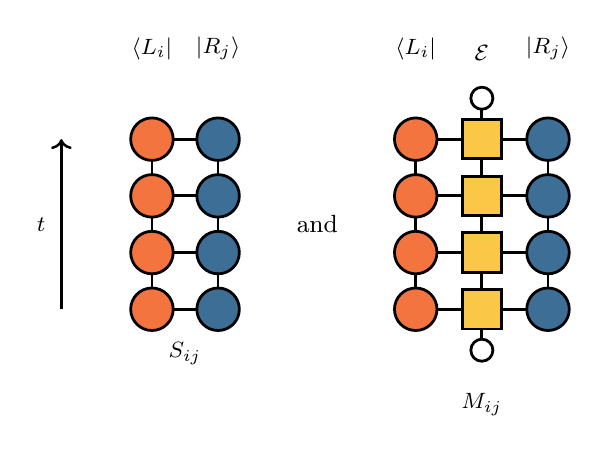
\begin{tikzpicture}[
    bond/.style={draw=black, line width=1.0pt},
    fat/.style={draw=black, line width=2.4pt},
    T/.style={circle, draw=black, line width=1.0pt, minimum size=5.4mm, inner sep=0pt},
    W/.style={rectangle, draw=black, line width=1.0pt, fill=tnE, minimum size=5.0mm, inner sep=0pt},
    P/.style={circle, draw=black, line width=1.0pt, fill=white, minimum size=2.8mm, inner sep=0pt},
    tag/.style={font=\small},
    idx/.style={font=\footnotesize},
  ]

  % product-state caps closing the tMPO column
  \newcommand{\caps}[1]{%
    \draw[bond] (#1,{1.5*\DY}) -- (#1,{1.5*\DY+0.52});
    \draw[bond] (#1,{-1.5*\DY}) -- (#1,{-1.5*\DY-0.52});
    \node[P] at (#1,{1.5*\DY+0.52}) {};
    \node[P] at (#1,{-1.5*\DY-0.52}) {};}

  % temporal MPS: #1 x, #2 fill, #3 leg side
  \newcommand{\tmps}[3]{%
    \draw[bond] (#1,{1.5*\DY}) -- (#1,{-1.5*\DY});
    \foreach \j in {-1.5,-0.5,0.5,1.5} {
      \draw[bond] (#1,{\j*\DY}) -- ({#1+(#3)*\LG},{\j*\DY});
      \node[T, fill=#2] at (#1,{\j*\DY}) {};
    }}

  % transfer-matrix column: legs on both sides, capped
  \newcommand{\tmpo}[1]{%
    \caps{#1}
    \draw[bond] (#1,{1.5*\DY}) -- (#1,{-1.5*\DY});
    \foreach \j in {-1.5,-0.5,0.5,1.5} {
      \draw[bond] ({#1-\LG},{\j*\DY}) -- ({#1+\LG},{\j*\DY});
      \node[W] at (#1,{\j*\DY}) {};
    }}

  % time axis: same direction as imgs/echo_strip.tex
  \draw[->, line width=0.9pt] (-1.15,{-1.5*\DY}) -- (-1.15,{1.5*\DY})
        node[midway, left=2pt, idx] {$t$};

  \tmps{0}{tnL}{1} \tmps{\CS}{tnR}{-1}
  \node[idx, anchor=south] at (0,{1.5*\DY+0.88})   {$\bra{L_i}$};
  \node[idx, anchor=south] at (\CS,{1.5*\DY+0.88}) {$\ket{R_j}$};
  \node[idx, anchor=north] at (0.42,{-1.5*\DY-0.30}) {$S_{ij}$};

  \node[tag] at (2.10,0) {and};

  \tmps{3.35}{tnL}{1} \tmpo{4.19} \tmps{5.03}{tnR}{-1}
  \node[idx, anchor=south] at (3.35,{1.5*\DY+0.88}) {$\bra{L_i}$};
  \node[idx, anchor=south] at (4.19,{1.5*\DY+0.88}) {$\mathcal{E}$};
  \node[idx, anchor=south] at (5.03,{1.5*\DY+0.88}) {$\ket{R_j}$};
  \node[idx, anchor=north] at (4.19,{-1.5*\DY-0.95}) {$M_{ij}$};

\end{tikzpicture}
\end{document}
.
\documentclass[tikz,border=3pt]{standalone}
\usepackage{amsmath,amssymb,braket,graphicx}
\usetikzlibrary{arrows.meta}

\definecolor{tnL}{RGB}{243,116,63}
\definecolor{tnR}{RGB}{60,110,150}
\definecolor{tnE}{RGB}{250,200,70}

\newcommand{\DY}{0.72}    % time-site spacing
\newcommand{\CS}{0.84}    % column spacing
\newcommand{\LG}{0.42}

\begin{document}
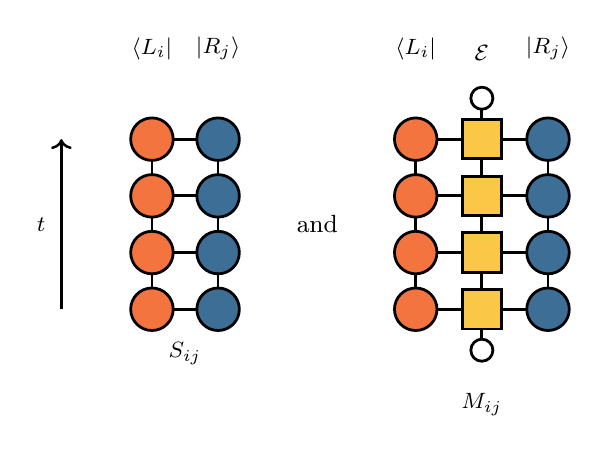
\begin{tikzpicture}[
    bond/.style={draw=black, line width=1.0pt},
    fat/.style={draw=black, line width=2.4pt},
    T/.style={circle, draw=black, line width=1.0pt, minimum size=5.4mm, inner sep=0pt},
    W/.style={rectangle, draw=black, line width=1.0pt, fill=tnE, minimum size=5.0mm, inner sep=0pt},
    P/.style={circle, draw=black, line width=1.0pt, fill=white, minimum size=2.8mm, inner sep=0pt},
    tag/.style={font=\small},
    idx/.style={font=\footnotesize},
  ]

  % product-state caps closing the tMPO column
  \newcommand{\caps}[1]{%
    \draw[bond] (#1,{1.5*\DY}) -- (#1,{1.5*\DY+0.52});
    \draw[bond] (#1,{-1.5*\DY}) -- (#1,{-1.5*\DY-0.52});
    \node[P] at (#1,{1.5*\DY+0.52}) {};
    \node[P] at (#1,{-1.5*\DY-0.52}) {};}

  % temporal MPS: #1 x, #2 fill, #3 leg side
  \newcommand{\tmps}[3]{%
    \draw[bond] (#1,{1.5*\DY}) -- (#1,{-1.5*\DY});
    \foreach \j in {-1.5,-0.5,0.5,1.5} {
      \draw[bond] (#1,{\j*\DY}) -- ({#1+(#3)*\LG},{\j*\DY});
      \node[T, fill=#2] at (#1,{\j*\DY}) {};
    }}

  % transfer-matrix column: legs on both sides, capped
  \newcommand{\tmpo}[1]{%
    \caps{#1}
    \draw[bond] (#1,{1.5*\DY}) -- (#1,{-1.5*\DY});
    \foreach \j in {-1.5,-0.5,0.5,1.5} {
      \draw[bond] ({#1-\LG},{\j*\DY}) -- ({#1+\LG},{\j*\DY});
      \node[W] at (#1,{\j*\DY}) {};
    }}

  % time axis: same direction as imgs/echo_strip.tex
  \draw[->, line width=0.9pt] (-1.15,{-1.5*\DY}) -- (-1.15,{1.5*\DY})
        node[midway, left=2pt, idx] {$t$};

  \tmps{0}{tnL}{1} \tmps{\CS}{tnR}{-1}
  \node[idx, anchor=south] at (0,{1.5*\DY+0.88})   {$\bra{L_i}$};
  \node[idx, anchor=south] at (\CS,{1.5*\DY+0.88}) {$\ket{R_j}$};
  \node[idx, anchor=north] at (0.42,{-1.5*\DY-0.30}) {$S_{ij}$};

  \node[tag] at (2.10,0) {and};

  \tmps{3.35}{tnL}{1} \tmpo{4.19} \tmps{5.03}{tnR}{-1}
  \node[idx, anchor=south] at (3.35,{1.5*\DY+0.88}) {$\bra{L_i}$};
  \node[idx, anchor=south] at (4.19,{1.5*\DY+0.88}) {$\mathcal{E}$};
  \node[idx, anchor=south] at (5.03,{1.5*\DY+0.88}) {$\ket{R_j}$};
  \node[idx, anchor=north] at (4.19,{-1.5*\DY-0.95}) {$M_{ij}$};

\end{tikzpicture}
\end{document}
.
\documentclass[tikz,border=3pt]{standalone}
\usepackage{amsmath,amssymb,braket,graphicx}
\usetikzlibrary{arrows.meta}

\definecolor{tnL}{RGB}{243,116,63}
\definecolor{tnR}{RGB}{60,110,150}
\definecolor{tnE}{RGB}{250,200,70}

\newcommand{\DY}{0.72}    % time-site spacing
\newcommand{\CS}{0.84}    % column spacing
\newcommand{\LG}{0.42}

\begin{document}
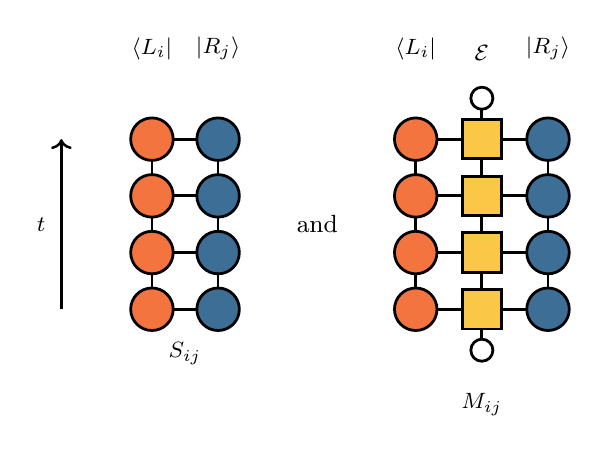
\begin{tikzpicture}[
    bond/.style={draw=black, line width=1.0pt},
    fat/.style={draw=black, line width=2.4pt},
    T/.style={circle, draw=black, line width=1.0pt, minimum size=5.4mm, inner sep=0pt},
    W/.style={rectangle, draw=black, line width=1.0pt, fill=tnE, minimum size=5.0mm, inner sep=0pt},
    P/.style={circle, draw=black, line width=1.0pt, fill=white, minimum size=2.8mm, inner sep=0pt},
    tag/.style={font=\small},
    idx/.style={font=\footnotesize},
  ]

  % product-state caps closing the tMPO column
  \newcommand{\caps}[1]{%
    \draw[bond] (#1,{1.5*\DY}) -- (#1,{1.5*\DY+0.52});
    \draw[bond] (#1,{-1.5*\DY}) -- (#1,{-1.5*\DY-0.52});
    \node[P] at (#1,{1.5*\DY+0.52}) {};
    \node[P] at (#1,{-1.5*\DY-0.52}) {};}

  % temporal MPS: #1 x, #2 fill, #3 leg side
  \newcommand{\tmps}[3]{%
    \draw[bond] (#1,{1.5*\DY}) -- (#1,{-1.5*\DY});
    \foreach \j in {-1.5,-0.5,0.5,1.5} {
      \draw[bond] (#1,{\j*\DY}) -- ({#1+(#3)*\LG},{\j*\DY});
      \node[T, fill=#2] at (#1,{\j*\DY}) {};
    }}

  % transfer-matrix column: legs on both sides, capped
  \newcommand{\tmpo}[1]{%
    \caps{#1}
    \draw[bond] (#1,{1.5*\DY}) -- (#1,{-1.5*\DY});
    \foreach \j in {-1.5,-0.5,0.5,1.5} {
      \draw[bond] ({#1-\LG},{\j*\DY}) -- ({#1+\LG},{\j*\DY});
      \node[W] at (#1,{\j*\DY}) {};
    }}

  % time axis: same direction as imgs/echo_strip.tex
  \draw[->, line width=0.9pt] (-1.15,{-1.5*\DY}) -- (-1.15,{1.5*\DY})
        node[midway, left=2pt, idx] {$t$};

  \tmps{0}{tnL}{1} \tmps{\CS}{tnR}{-1}
  \node[idx, anchor=south] at (0,{1.5*\DY+0.88})   {$\bra{L_i}$};
  \node[idx, anchor=south] at (\CS,{1.5*\DY+0.88}) {$\ket{R_j}$};
  \node[idx, anchor=north] at (0.42,{-1.5*\DY-0.30}) {$S_{ij}$};

  \node[tag] at (2.10,0) {and};

  \tmps{3.35}{tnL}{1} \tmpo{4.19} \tmps{5.03}{tnR}{-1}
  \node[idx, anchor=south] at (3.35,{1.5*\DY+0.88}) {$\bra{L_i}$};
  \node[idx, anchor=south] at (4.19,{1.5*\DY+0.88}) {$\mathcal{E}$};
  \node[idx, anchor=south] at (5.03,{1.5*\DY+0.88}) {$\ket{R_j}$};
  \node[idx, anchor=north] at (4.19,{-1.5*\DY-0.95}) {$M_{ij}$};

\end{tikzpicture}
\end{document}
